\chapter{Renderering}

在渲染方面上的研究与优化已经发展成熟,已成为一个非常复杂的系统了,本文的目标是从理解渲染的技术原理,从软渲染,到CPU,再到GPU。
为简化,我们以图元三角形为例,主要有两个阶段:
\begin{itemize}
    \item {决定那些像素坐标构成这个三角形}
    \item {决定这些像素的颜色值是多少,这个过程就是着色shading}
\end{itemize}
它们分别对应着图形学中另外两个概念,光栅化和光照模型。

\section{Rasterize}
光栅化
图形学中,是物理的三维世界,如何把三维物体在二维屏幕上显示,需要把它的三维属性都降为二维的结果,大致存在以下几个步骤:

\begin{itemize}
    \item {坐标变换}
    \item {属性计算,如颜色,纹理,alpha等}
    \item {光栅化}
\end{itemize}

\textsf{目前大众屏幕分辨率为1920x1080,在二维屏幕渲染时,内存中的FrameBuffer只保存着1920x1080个屏幕点的颜色,然后再映射到屏幕上面。
光栅化的,就是计算出1920x1080个点的颜色值的过程。把物体的数学描述转换为屏幕的像素值,是从连续到离散,即物理的坐标是浮点数,而屏幕坐标是整数,光栅化的过程是一个近似的过程。
在一些图形处理软件中就是把矢量图形转化成像素点的过程。}

\begin{description}
    \item [主动:] \textsf{定时渲染,与时间关系比较严格的}
    \item [被动:] \textsf{请求渲染,与动画相关的,以流畅为结果}
\end{description}

\text{目前处理光照生成图像的过程中,计算的级别有:}

\begin{itemize}
    \item {逐顶点光照,在每个顶点计算光照,在渲染图元内部进行插值,光照模型中的非线性关系会产生问题}
    \item {逐像素光照,Phong着色,在fragment对顶点法线进行插值}
\end{itemize}


\section{Photorealistic Rendering}

真实感图形技术包括消隐技术,光照模型,明暗处理和纹理,阴影生成等

\begin{itemize}
    \item {局部光照,仅处理光源直接照射物体表面的光照模型,与光栅化渲染算法相适应的,一次只考虑
    一个像素的光照强度,逐像素的光照计算,不能得到其他像素的光照影响值}
    \begin{itemize}
        \item {Lambert漫反射模型,不能很好处理镜面与高光}
        \item {Gourand}
        \item {Phong,支持高光与镜面}
        \item {Blinn-Phong,速度快,目前商业普遍使用}
        \item {Cook-Torrance,以双向反射的基础上}
    \end{itemize}
    \item {全局光照,基于光学物理原理,光照强度的计算依赖于光能在现实世界中的传播,考虑光线与整个场景中
    各物体表面以及物体表面之间的相互影响,包括多次反射、透射、散射等,成熟应用在离线渲染中}
    \begin{itemize}
        \item {光线跟踪,模拟光从光源出发经过若干次反射、折射达到摄像机的过程,由于只有最终到达摄像机的光线
        才对生成图像有贡献,实现中是以摄像机逆向发出光线,以寻求达到光源的路径。}
        \begin{itemize}
            \item {路径跟踪Path Tracing}
            \item {递归光线追踪Whitte-type}
            \item {分布式光线追踪Distrubution}
            \item {双向路径追踪Bidirectional Path}
            \item {Metropolis}
        \end{itemize}
        \item {辐射度算法,是一种物体空间的算法,用于解离散点或环境中表面曲面面片的光强度问题,而不是解图像平面
        投影的像素问题}
        \item {光子映射,改善漫反射辉映,焦散等全局光照效果,还无法应用在实时渲染中}
    \end{itemize}
\end{itemize}

\section{Non-Photorealistic Rendering}
对于某些场景,不需要真实感,需要一些艺术化的表现
钢笔素描的生成,
中国国画与书法的生成。
\newline
\textbf{Artistic Shading},艺术渲染,模拟人简画的素描之类的,是一种根据轮廓来来抽象效果。

\section{Image-Based Rendering}

IBR,基于图像的渲染,完全摒弃传统的先建模,然后确定光源的渲染方法,
它直接从一系列已知的图像中生成新颖的视口图像,适用于野外极其复杂场景的生成和漫游。

\section{Stereo Rendering}
立体渲染,是一种让人眼能够感受到立体效果的渲染方式,需要两个camera对同一个场景进行渲染,两个view得到
的图像略有差异(两个camera的投影矩阵的差异),让人产生深度的视觉效果。一般分左右两个camera。

通常渲染完成后,整张图像还需要一次后处理Barrel distortion桶形失真,以抵消VR设备固有的pincushion distortion枕形失真。
\begin{figure}[h]
    \centering
    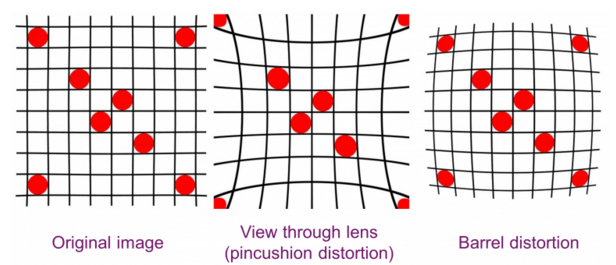
\includegraphics[width=\textwidth]{images/Optimising-OpenGL-ES-for-mobile-VR-lens-distortion.png}
    \caption{Phong Shading Model}
\end{figure}

\chapter{Illumination Model}

当光照射到物体表面时,物体会对光发生反射、透射、吸收、衍射、折射、干涉等。其中被物体吸收的部分转化为热。
反射、透射的光会进入人的视觉系统,使我们看见物体。为了模拟仿真这一真实的现象,建立一些数学模型来替代复杂的真实
物理模型,这些模型就称为光照模型。

\section{Lamertian}
1970年Bouknight提出了第一个光反射模型。1971Gourand提出“漫反射模型+插值”的思想,称为Gourand明暗处理。
即出物体表面朝向(即法线)是确定物体表面上一点光强的主要因素,用Lambert漫反射定律计算物体表面上各多
边形的光强,对光照射不到的使用环境光代替。
\textbf{Lambert's cosin law},告诉我们曲面表面的颜色c与表面法线和光源方向的夹角的余弦值cosine成正比。

\begin{align*}
c \propto cos(\theta) \\
c \propto n \cdot l 
\end{align*}

漫反射:当光线从光源照射到曲面表面时,表面向每个方向散射辐射量。漫反射符合兰伯特定律。

\begin{align*}    
c_{diffuse} = max(0, \hat{n} * \hat{l}), \\
c_{ambient} = Kd * Ia, \\
c_{light} = Kd * Il, \\ 
c_{final} = c_{ambient} + c_{light}c_{diffuse}, \\
0 < Kd < 1, 
\end{align*}

Kd是材质对环境光的反射系数,Ia表示环境光强度,Il表示点光源强度
注意,这里存在一个前提,就是假设光源方向l不依赖渲染物体的位置信息,就是光与渲染对象有足够的远,就是
方向光directional light。

\section{Phong Model}

Phong模型引入镜面光,即ADS(ambient,diffuse,specular),认为镜面与反射的光强和反射光线与视线的夹角相关

\begin{figure}[htbp]
    \centering
    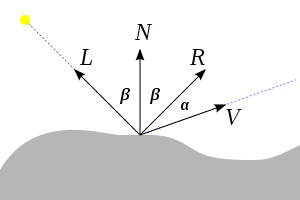
\includegraphics[width=0.8\textwidth]{images/phong-shading-model.png}
    \caption{Phong-Model-Specular}\label{Phong-Model-Specular}
\end{figure}

图\ref{Phong-Model-Specular}中的$\alpha$ 很小时,就是高光效果

\begin{align*}
    R = -L + 2(L \cdot N) * N \\
    I_{spec}=Ks * Il * (dot(V, R))^N_{s}
\end{align*}

Ks为镜面反射系数,Ns为高光指数。
Blinn-Phong是基于Phong的修正模型,

\begin{align*}
    H = \frac{L + V}{|L + V|}, \\
    I_{spec} = Ks * Il * (dot(N, H))^N_{s}
\end{align*}

H是入射光线方向L与视线方向V的中间向量,称之为半角向量。相比两者,前者更真实,后者高光更柔和,且计算速度较快,
实际中应用更广,OpenGL和DirectX渲染管线中是默认渲染模型。

\section{Global Illumination}
现实中的物体表面会接收大部分或全部来自其他反射出来的光线,称为indirect lighting或mutual illumination。
局部光照模型只考虑光对物体的照明,忽略了物体间的相互影响,其一般公式可以表示为

\begin{align*}
    I = I_{abmient} + \sum_{i}^{N}I_{light}\frac{1}{k_{c}+k_{l} \cdot d_{i} + k_{q} \cdot d_{i}^2}
    \left[ k_{d}(N \cdot L) + k_{s}(R \cdot V)^n \right]
\end{align*}

每个光源对物体的影响主要包括漫反射和镜面反射两部分,局部照明的阴影算法需要单独考虑。
\newline
全局照明考虑更全面,它自带阴影效果。它主要有两种算法:
\begin{itemize}
    \item {光线追踪法, 关注于镜面反射光,可严格追踪反射光线的方向,实际中采用逆向追踪法,减少计算量}
    \item {辐射度法, 关注于漫反射光,}
\end{itemize}
基本模型是 
\newline

\begin{align*}
    I_r = I_{ia}R_{a} + \sum_{l}I_{il}(N \cdot L_{l})d \omega_{il}(sR_{s} + dR_{d})
\end{align*}

其中的环境光和漫反射分量不依赖于观察者的位置View's Position。假设表面是由微面元组成microfacet,其镜面分量为:
\newline

\begin{align*}
    R_s = \frac{F}{\pi} \frac{DG}{\pi (N \cdot L)(N \cdot V)}
\end{align*}

为更加丰富,引入了几何项G,Fresnel项F,粗糙度项D。
\newline

\textbf{粗糙度项D},代表了可以有效反射光的那一部分微面元所占的比例,有多种分别函数。
高斯分布模型
\newline

\begin{align*}
    D = ce^{-(\alpha / m)^2}
\end{align*}

Bechmann分布函数
\newline

\begin{align*}
    D = \frac{1}{m^2cos^4(\theta)}e^-(tan\alpha / m)^2
\end{align*}

\textbf{几何项G},几何衰减项,表现了微小面元之间的互相遮挡shadowing and masking所造成的影响。
\newline

\begin{align*}
    G = \left\{
        1, \frac{2(N \cdot H)(N \cdot V)}{(V \cdot H)}, \frac{2(N \cdot H)(N \cdot L)}{(V \cdot H)} 
    \right\}
\end{align*}

\textbf{Fresnel项F},描述了在每一个微面元上光是如何反射,与入射角和波长相关。
\newline

\begin{align*}
    c = cos(\theta) = V \cdot H \\
    g^2 = n^2 + c^2 - 1 \\
F = \frac{1(g-c)^2}{2(g+c)^2} \left\{ 1+\frac{[c(g+c)-1]^2}{[c(g-c)+1]^2} \right\}
\end{align*}

\section{Physically based Rendering}

PBR refers to the concept of using realistic shading/lighting models along with measured surface values to accurately represent real-world materials

\chapter{Texture}

可阅读
Chapter 20 Textures and Texture Mapping\cite{CGPP3ed}

Chapter 11 Texture Mapping\cite{FCG4ed}

Chapter 6 Texturing\cite{RTR4ed}

纹理应用在表面的大致逻辑是
\begin{lstlisting}
    Color texture_lookup(Texture t, float u, float v) {
        int i = round(u * t.width() - 0.5);
        int j = round(v * t.height() - 0.5);
        return t.get_pixel(i,j);
    }
    Color shade_surface_point(Surface s, Point p, Texture t) {
        Vector normal = s.get_normal(p);
        (u,v) = s.get_texcoord(p);
        Color diffuse_color = texture_lookup(t, u, v);
        // compute shading using diffuse_color and normal 
        // return shading result    
    }
\end{lstlisting}

\section{Texture Coordinate}
 纹理坐标的生成.

以顶视图Y轴方向来看,对X(S)和Z(T)生成对应的纹理坐标值UV,即Y平面为UV展开

\begin{enumerate}
    \item \textsf{遍历所有点得到lowestX和highestX,lowestX=-12.00,highestX=134.56}
    \item \textsf{得到绝对范围 range=(lowest - highest) * -1 = (-12.00-134.56)*-1=146.56}
    \item \textsf{与0的偏移值offset=0-lowestX=0 - (-12.00)=12}
    \item \textsf{vertex x=87.45, absoluteX=X+offset=87.45+12=99.45}
    \item \textsf{get S value, s = absoluteX / range = 99.45/145.56=0.679}
    \item \textsf{do the same for Z axis to get T value}
\end{enumerate}

由Image Space得到Texture space T, 存在一个函数映射Surface S in World space, 数学模型如下:

\begin{align*}
    \phi &: S \rightarrow T \\
    &: (x,y,z) \rightarrow (u,v)
\end{align*}

函数$\phi$存在很多种形式

\subsection{Planar Projection}

orthographic viewing $M_{t}$是变换矩阵

\begin{align*}
    \phi(x,y,z) = (u,v) \qquad where 
    \begin{bmatrix} u \\ v \\ * \\ 1 \end{bmatrix} = M_{t} 
    \begin{bmatrix} x \\ y \\ z \\ 1 \end{bmatrix}
\end{align*}

perspective viewing $P_{t}$是投影矩阵

\begin{align*}
    \phi(x,y,z) = (u/w,v/w) \qquad where 
    \begin{bmatrix} u \\ v \\ * \\ w \end{bmatrix} = P_{t} 
    \begin{bmatrix} x \\ y \\ z \\ 1 \end{bmatrix}
\end{align*}


\subsection{Sphereical Coordinates}

\begin{equation}
    \phi(x,y,z) = ([\pi+atan2(y,x)]/2\pi,[\pi-acos(z/s\|x\|)]/\pi)
\end{equation}

\subsection{Cylindrical Coordinates}

\begin{align*}
    \phi(x,y,z) = (\frac{1}{2\pi}[\pi+atan2(y,x)]/2\pi,\frac{1}{2}[1+z])
\end{align*}

\subsection{Cubemaps}

\begin{align*}
    \phi(x,y,z) \mapsto (\frac{x}{z},\frac{y}{z})
\end{align*}

\subsection{Interpolated Texture Coordinates }

\begin{description}
    \item [distortion] \textsf{映射关系是一个连续的函数,就存在失真,扭曲,畸变}
    \item [seam] \textsf{拓扑可以展开为平面,但是因为顶点可能有多个uv值,会出现缝隙问题,边界过渡问题}
\end{description}

\subsection{UV Unwrapping}

UV展开就是把物体的表面映射到平面图像上的过程。为了让弯曲的表面信息也能在平面上被精准存放下来,对切割线seam的要求

\section{Bump Map}

为增加表面法向量细节,如一个平面法向量处处相同,即时使用纹理,光照效果仍然不够真实,可以增加扰动表面面皮的法向量,
从而形成比较真实的效果。

纹理贴图存储的是颜色值,而Bump Map存储的是凹凸数据,通常是高度值。
Bump Map是Phong Shading的一项扩展,因为表面法线用来计算顶点的光亮,而Bump Map就是为了影响法线的改变,最终影响颜色值。
所以算是一种负责光方向的纹理映射,不同的凹凸数据,使用不同的方法来影响法线。

\begin{itemsize}
    \item \text{Emboss Bump Map}
    \item \text{DOT3 Bumap Map}
\end{itemsize}

\subsection{Normal Map}

是实时渲染中,通常使用凹凸贴图的变种法线贴图,bluish texture偏蓝色纹理,法线贴图在纹理的每个像素中存储一个颜色。
有两种方法生成法线贴图
\begin{itemize}
    \item \text{灰度图,预先计算每个像素与其垂直和水平相邻像素之间的差别,将两个结果数字(导数)转换为单位法线并存储为颜色}
    \item \text{精模烘焙法线,把纹理的每个像素与精模的表面位置结合起来,将其结果编码为法线存储为颜色值}
\end{itemize}

为使生成的纹理可以在任意旋转下均反复使用,存储的法线必须在\textbf{切线空间}中,切线空间由三个向量normal法线,tangent切线,binormal副法线组成。
切线空间决定了表面的朝向。

切线空间的映射依赖物体的UV纹理,因为UV纹理中的决定世界空间中的切线空间的两个向量,切线和副法线。
生成较好的UV纹理在切线空间中不穿帮是比较困难和耗时的。

\subsection{Height Map}
高度图是存储高度信息的数据,通常计算XY方向上的倾斜度

\begin{gather*}
    x_gradient = pixel(x-1,y) - pixel(x+1,y) \\
    y_gradient = pixel(x,y-1) - pixel(x,y+1) \\
    normalNew = normal + (U * x_gradient) + (V * y_gradient)
\end{gather*}

在的Bump Map\cite{CGPP3ed}中,有一个公式更加通用

\begin{align*}
    n^{'} = S(n + rt_{1} + gt_{2})
\end{align*}

它描述了两个方向上向量对法线的影响


\chapter{Shadow}

目前的阴影是模拟的效果,在非物理渲染中就是

\section{Shadow Map}

运用渲染到纹理方法render to target,以场景中的光源为坐标原点,建立光源坐标系,就是场景深度
把render target(一般是R32F的surface)就是Shadow Map。 

接着正常render frame buffer, 启用depth buffer,将场景中的世界坐标的物体转化到以光源为基准的
投影坐标系中

世界坐标 $\rightarrow$ 物体坐标 $\rightarrow$ 光源坐标 $\rightarrow$ 光源视图坐标 $\rightarrow$ 光源投影坐标

任何在fragment shader中比较深度值,深度值小于shadow map对应的深度,就是光源照射地方,否则就是照射不到地方。
比较深度值时要把坐标转换为窗口坐标,因为shadow map是render to target的surface的结果。

\begin{itemize}
    \item [优点] \text{不用像volume那样去计算所有对象形状,只产生一直map}
    \item [缺点] \text{阴影有锯齿,比较深度值时就两种值,有阴影1和无阴影0,在阴影的边缘0和1交替出现而产生锯齿}
\end{itemize}

\subsection{PCF}

Perecentage Closer Filter, 将深度比较的结果0和1存储在一个render target里面,然后对其进行过滤操作,
产生值为0.2,0.5,...等灰度值的,即soft shadow。消耗时间较长,就简化成横向或纵向过滤,减少采样数量。

\subsection{CSM}

convolution shadow map, 此方法基于阴影重建,深度值比较的结果要么是1,要么是0,从而构造一个x坐标为[-1,1],
y坐标为[0,1]的函数,对函数进行FFT变换,运用基准函数sin和cos来重新构建shadow map。 

\subsection{VSM}

variance shadow map, 此方法应用切尔雪夫不等式,


\chapter{Algorithm}
记录一些算法和思路

\section{Camera}

\begin{figure}[h]
    \centering
    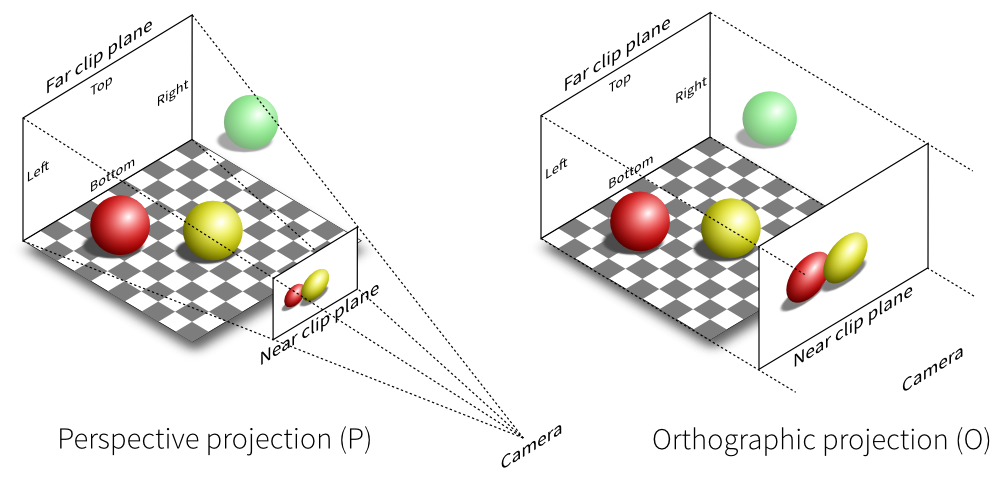
\includegraphics[width=1\textwidth]{images/camera-perspective-and-orthographic.png}
    \caption{左边:透视投影;右边:右边正交投影}    
\end{figure}

\subsection{Perspective Best-Fit}
关于camera的自动对焦算法,对透视camera有: side是bounding box的最大边, distance是从camera的位置到bounding box的中心距离

\begin{align*}
    tan(\alpha / 2) = \frac{(side / 2)}{distance}
\end{align*}

对应的threejs的代码如下:

\begin{lstlisting}
    let box = calculateBoundingBoxInScene();
    let center = new THREE.Vector3(), size = new THREE.Vector3();
    box.getCenter(center); box.getSize(size);
    let maxSide = Math.max(size.x, Math.max(size.y, size.z));    
    let distance = maxSide /
         ( 2 * Math.tan(THREE.Math.DEG2RAD * alpha / 2));  
    camera.position.set(center.x, center.y, center.z - distance);
    camera.position.z *= Math.sqrt(3);
\end{lstlisting}

\subsection{Perspective Side}



\section{ Edge Function }
Juan Pineda \cite{EdgeFunction} 在他论文提出的概念,就是\textbf{barycentric coordinates}的应用。
它在计算三角形属性方面上有很大的优势,如深度z-depth、颜色color、纹理坐标uv、法线等插值计算。
重心(质心)坐标的应用主要体现在:
\begin {itemize}
    \item {判断一个点是否在三角形内}
    \item {根据三角形三个顶点得到三角形内一个点P}
\end {itemize}
在软光栅化或光线追踪都用得到。

\begin{figure}[h]
    \centering
    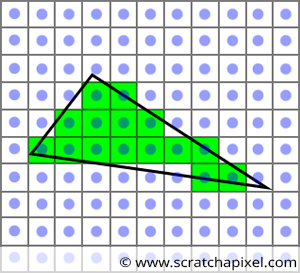
\includegraphics[width=0.25\textwidth]{images/rasterization-triangle1.png}
    \hspace{0.1cm}
    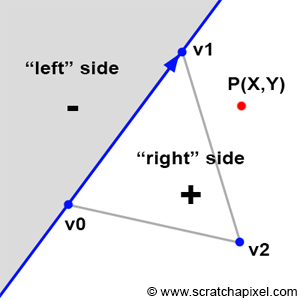
\includegraphics[width=0.25\textwidth]{images/rasterization-triangle2.png}
    \hspace{0.1cm}
    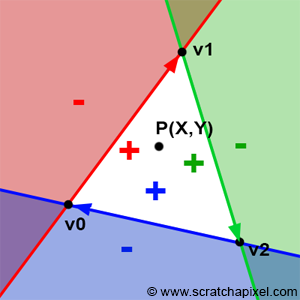
\includegraphics[width=0.25\textwidth]{images/rasterization-triangle3.png}
    \caption{左边:测试像素是否覆盖三角形,是光栅化算法的原理;
    中间:判断点与线的关系,大于0在右边,小于0在左边,等于0在线上;
    右边:在白色区域中的点都是位于三角形边的右边
    }    
\end{figure}
遍历整个FrameBuffer去判断点是不是在在三角形内部,太浪费时间去遍历不可能的结果了。
\begin{figure}[h]
    \centering
    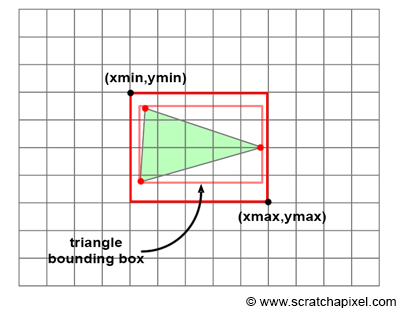
\includegraphics[width=0.3\textwidth]{images/rasterization-boundingbox.png}
    \caption {三角形的顶点告诉了大致范围,减少遍历的次数,提高访问性能}
\end{figure}
计算boundingbox的算法很简单,速度也快。

\section{Reconstructing Position From Depth}
需求:根据当前像素的Depth计算出View空间中的Position
先分析depth是如何计算出来的,在vertex shadeer中
\begin{lstlisting}
    outPos = mul(inPos, mvp);
    outDepth.xy = outPos.zw;
\end{lstlisting}
在pixel shader中,
\begin{lstlisting}
    depth = outDepth.x / outDepth.y;
\end{lstlisting}
按照这个过程逆运算回去
\begin{lstlisting}
    z = texture(depthSampler, inUV);
    x = inUV.x * 2 - 1;
    y = (1 - inUV.y) * 2 - 1;
    pos = (x,y,z,1)
    pos = mul(pos, mvpInverse);
    pos = pos.xyz / pos.w;
\end{lstlisting}
但是存在一些问题
\begin{itemize}
    \item {z/w是非线性分布的,经过RTT(Render To Texture)后再变换回去,精度存在误差}
    \item {计算量大}
\end{itemize}
从物理状态来看看摄像机的视锥体的抽象形式,从摄像机位置到远裁剪面发射一条射线,存在一个关系:

\begin{figure}[h]
    \centering
    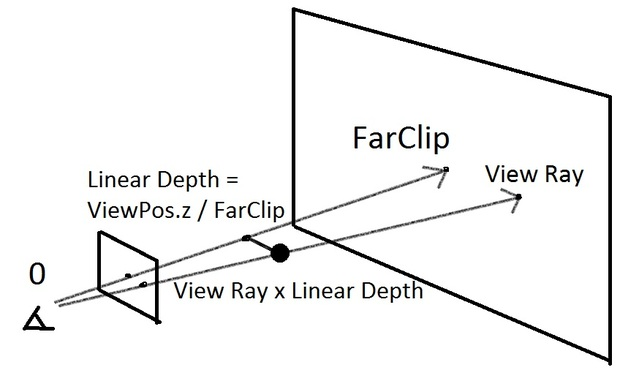
\includegraphics[width=0.5\textwidth]{images/reconstructing-position-from-depth.png}
\end{figure}

\begin{lstlisting}
    posView = viewRayDir * linearDepth;    
    linearDepth = posView.z / farClipDistance;
\end{lstlisting}

linearDepth是规格化的Z值,它满足线性分布。现在的问题就如何得到RayDir向量了。在View空间中,摄像机的位置是(0,0,0),
对于可见的每个点,从摄像机出发的射线都与远裁剪面相交,交点就是方向向量RayDir的坐标。由图中可知,是利用中心线和射线组成的三角形,满足等比关系,是线性关系。
远裁剪面的四个顶点是可以计算出来的,思路就出来了。

\begin{itemize}
    \item {1. 把posView.z/farClipDistance的值保存到RTT中,得到的值满足线性关系}
    \item {2. 从RTT中得到linearDepth, 从vertex shader中得到viewRayDire.xy, }
\end{itemize}

\begin{lstlisting}
    viewRayDir = float3(farClip.x, farClip.y, farClipDistance);
    posView = viewRayDir * linearDepth;
\end{lstlisting}

\section{Trackball}
轨迹球\cite{Trackball}
轨迹球就是在屏幕之外虚构一个球形曲面,使鼠标在二维屏幕上的移动投影到球形曲面上。
即一个半球覆盖在屏幕上面。以屏幕中心为球心O,X轴向右,Y轴向上,Z轴向外。当鼠标在球面的范围内移动时,可以由二维屏幕上的二维左边点P(x,y),通过数学关系求得其在球面上的投影点P'。
鼠标从P1移动到P2,对应的球面就是从P1'到P2'。产生两个向量V1=OP1',V2=OP2',  
V1与V2的叉乘得到向量N,即三维物体的旋转轴,V1到V2的转角量就是三维物体的旋转角度。
屏幕时矩形,球形的投影在屏幕的平面上只会是一个圆,总会有些区域的点投影后会落在球面之外。

\section{Grid}
绘制网格,是很多场景都需要的,有两种思路, 基于直线,基于Pattern网格思路。
直线的思路就是一个plane效果。而Pattern的网格思路是一个模式,更符合screen效果。
\begin{lstlisting}
    uniform vec2 pitch; // unit-x, unit-y
    uniform float scale; // 10

    float offsetX = gl_FragCoord.x;
    float offsetY = 1.0 - gl_FragCoord.y;
    if (int(mod(offsetX, pitch[0])) == 0 || int(mod(offsetY, pitch[1])) == 0) {
        if (int(mod(offsetX, pitch[0] * scale)) == 0 || int(mod(offsetY, pitch[1] * scale)) == 0) {
            gl_FragColor = vec4(0.8, 0.8, 0, 0.5);
        } else {
            gl_FragColor = vec4(0.8, 0, 0, 0.5);
        }
    } else {
        discard;
    }
\end{lstlisting}

